\part{Phase Two: Implement Client with HTLM5, CSS3 and JS}

\chapter*{Introduction}
\label{c_phasetwo}
On this section, we will experiment with different frameworks to improve the
tool in terms of UX and functionality. Also we will look for new ways to show
same data, just following a Lean approach and go step by step until the result
is the successful one.


\chapter{Facelift with Bootstrap}
There are few front end frameworks that help the web developer to build a
consistent, usable and responsive web, such as
Backbone\footnote{\url{http://backbonejs.or}}, 
Underscore\footnote{\url{http://underscorejs.org/}},
Skeleton\footnote{\url{http://www.getskeleton.com/}},
Foundation\footnote{\url{http://foundation.zurb.com/}},
Compass\footnote{\url{http://compass-style.org/}},
Bootstrap\footnote{\url{http://getbootstrap.com/}} and few others. With them
you cover the required features to build a web tool in a
single page and/or have responsive mobile web implementation using the latest
CSS3 and Saas extension, like Compass.

I started applying Bootstrap to the dashboard in a very straightforward way and
getting awesome results a couple of hours later.

First thing to do is to import required libraries, such as main style sheet,
JavaScript extensions (that is required to get some fancy actions and effects)
and optional theme, as it is shown on the following code
\ref{f_facelift_bootstrap_code}, note that the library is loaded from the
closest server to the user as it is using \emph{MaxCDN.com} service
(\texttt{//maxcdn.bootstrapcdn.com/\ldots}), being a distributed replication
content system\footnote{Other similar system would be
\url{http://www.akamai.com}.}.

\begin{lstlisting}[style=html,breaklines=true,caption=Bootstrap\
required\ libraries,label=f_facelift_bootstrap_code]
<!-- Bootstrap http://getbootstrap.com/getting-started/ --> 
<!-- Latest compiled and minified CSS --> 
<link rel="stylesheet" href="//maxcdn.bootstrapcdn.com/bootstrap/3.2.0/css/bootstrap.min.css">

<!-- Optional theme -->
<link rel="stylesheet" href="//maxcdn.bootstrapcdn.com/bootstrap/3.2.0/css/bootstrap-theme.min.css">

<!-- Latest compiled and minified JavaScript -->
<script src="//maxcdn.bootstrapcdn.com/bootstrap/3.2.0/js/bootstrap.min.js"></script>
<!-- Bootstrap -->
\end{lstlisting} 

Once we have the style sheet loaded, we just need to apply to our html entities
the proper class and role and result is just so fancy as you can see on the
following \reffigure{f_facelift_bootstrap},
\reffigure{f_facelift_bootstrap_2} and \reffigure{f_facelift_bootstrap_3}.

\begin{figure}[ht!]
	\centering
   	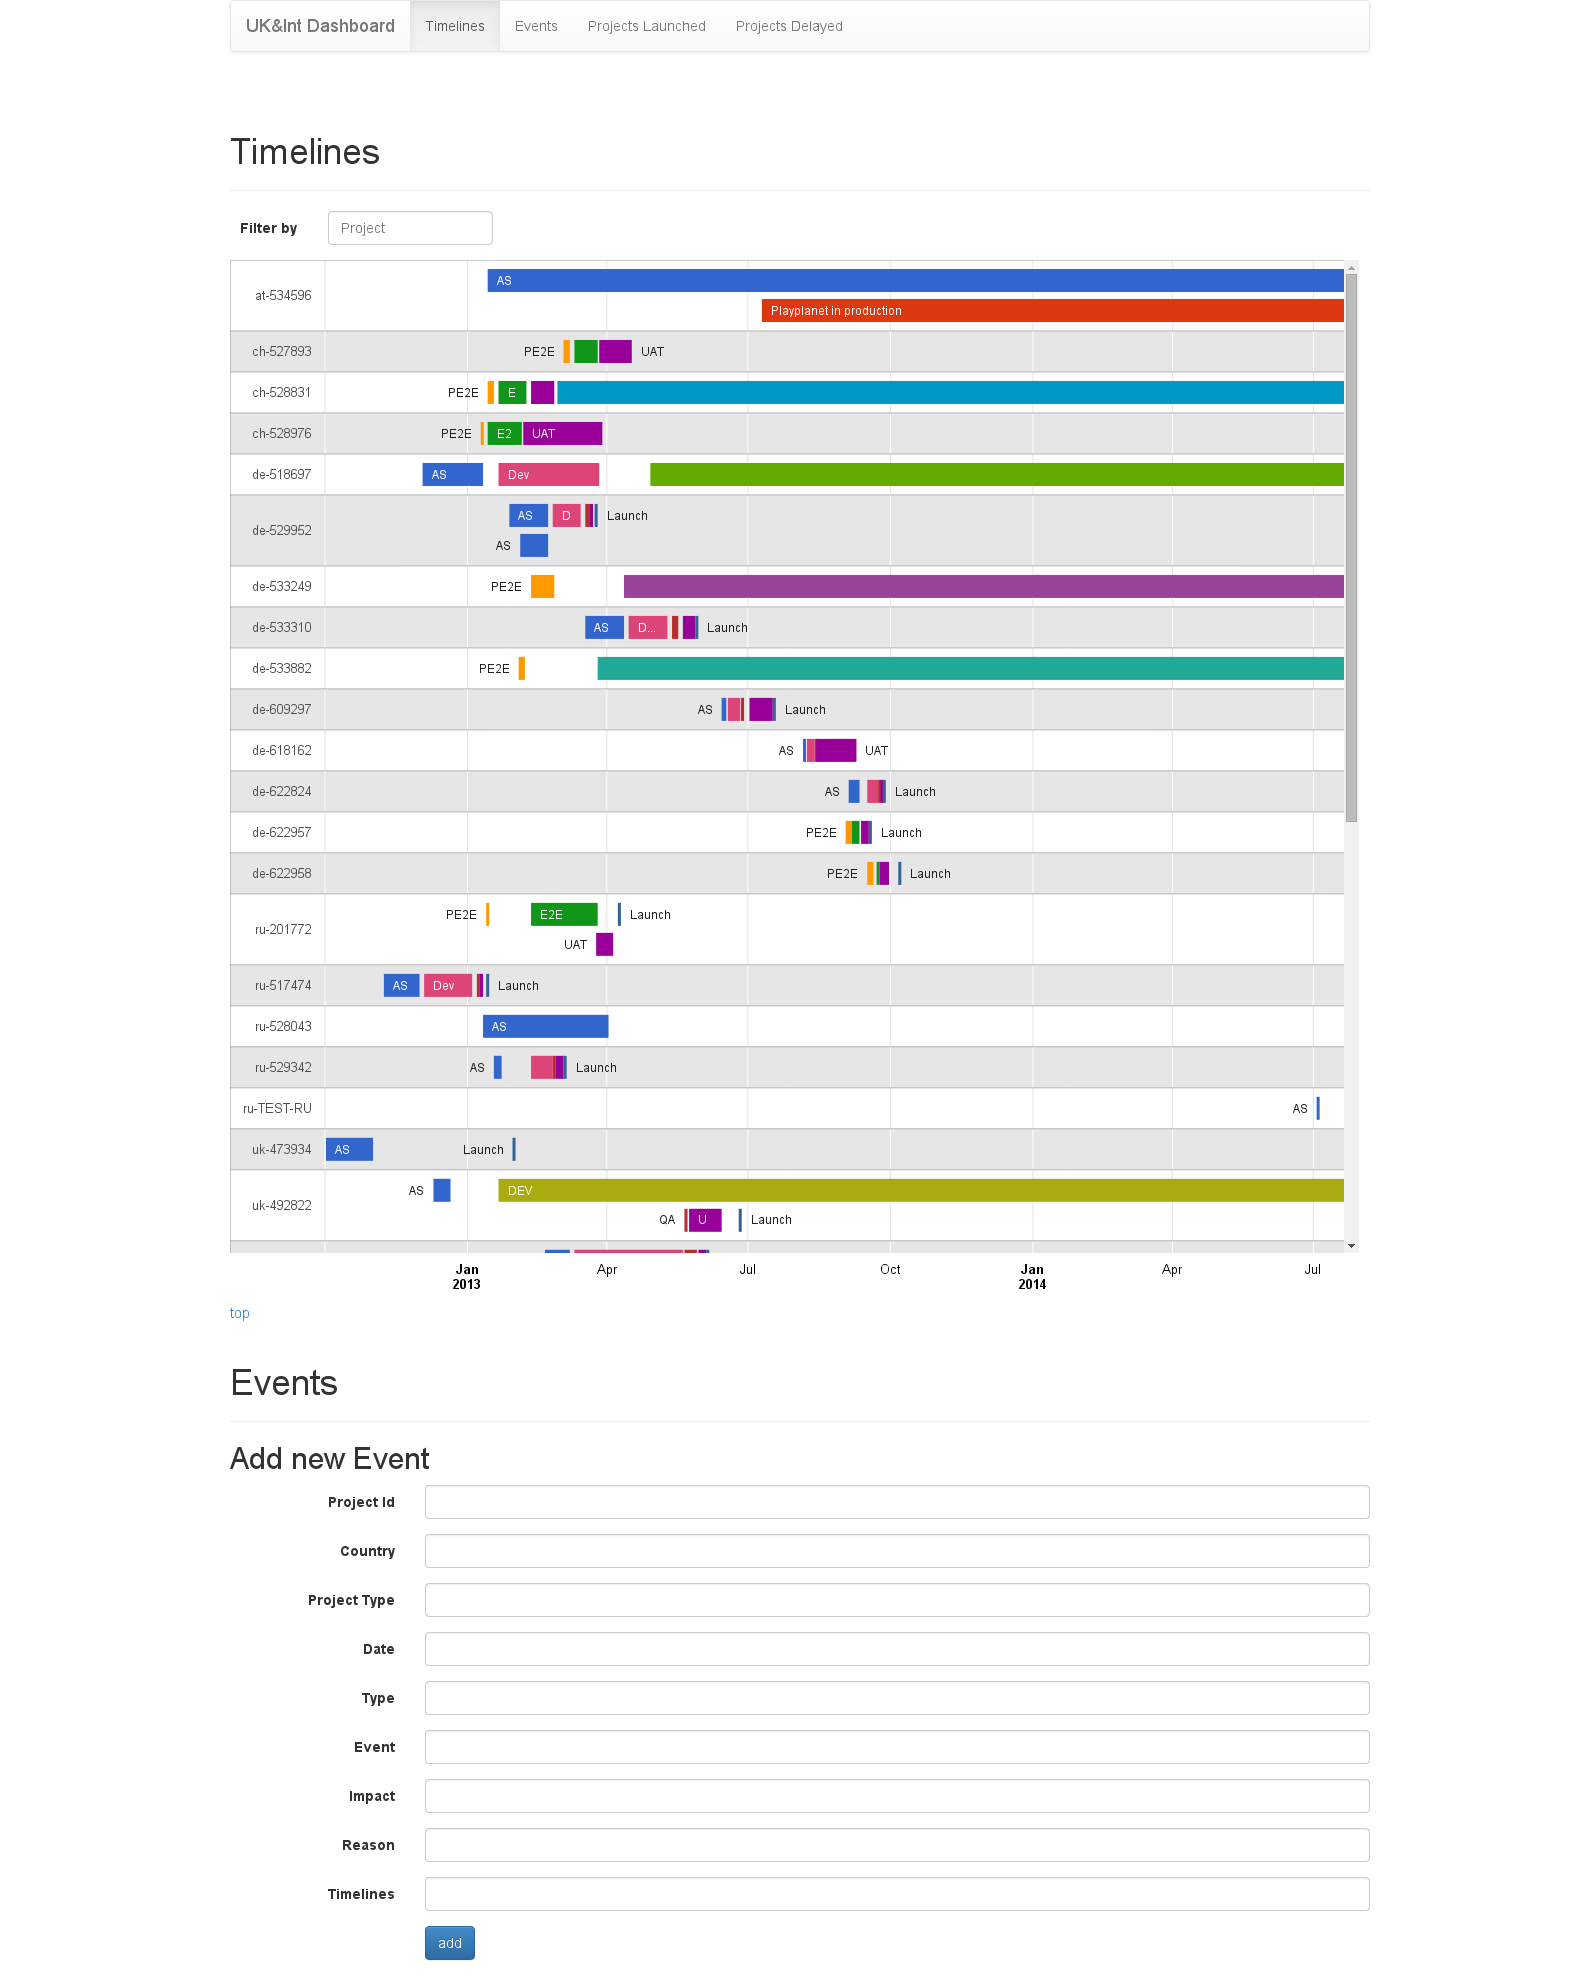
\includegraphics[width=1\textwidth]{./resources/dashboard_after_bootstrap_1.png}
   	\caption{Dasboard look and feel after apply Bootstrap style sheet (1)}
   	\label{f_facelift_bootstrap}
\end{figure}

\begin{figure}[ht!]
	\centering
   	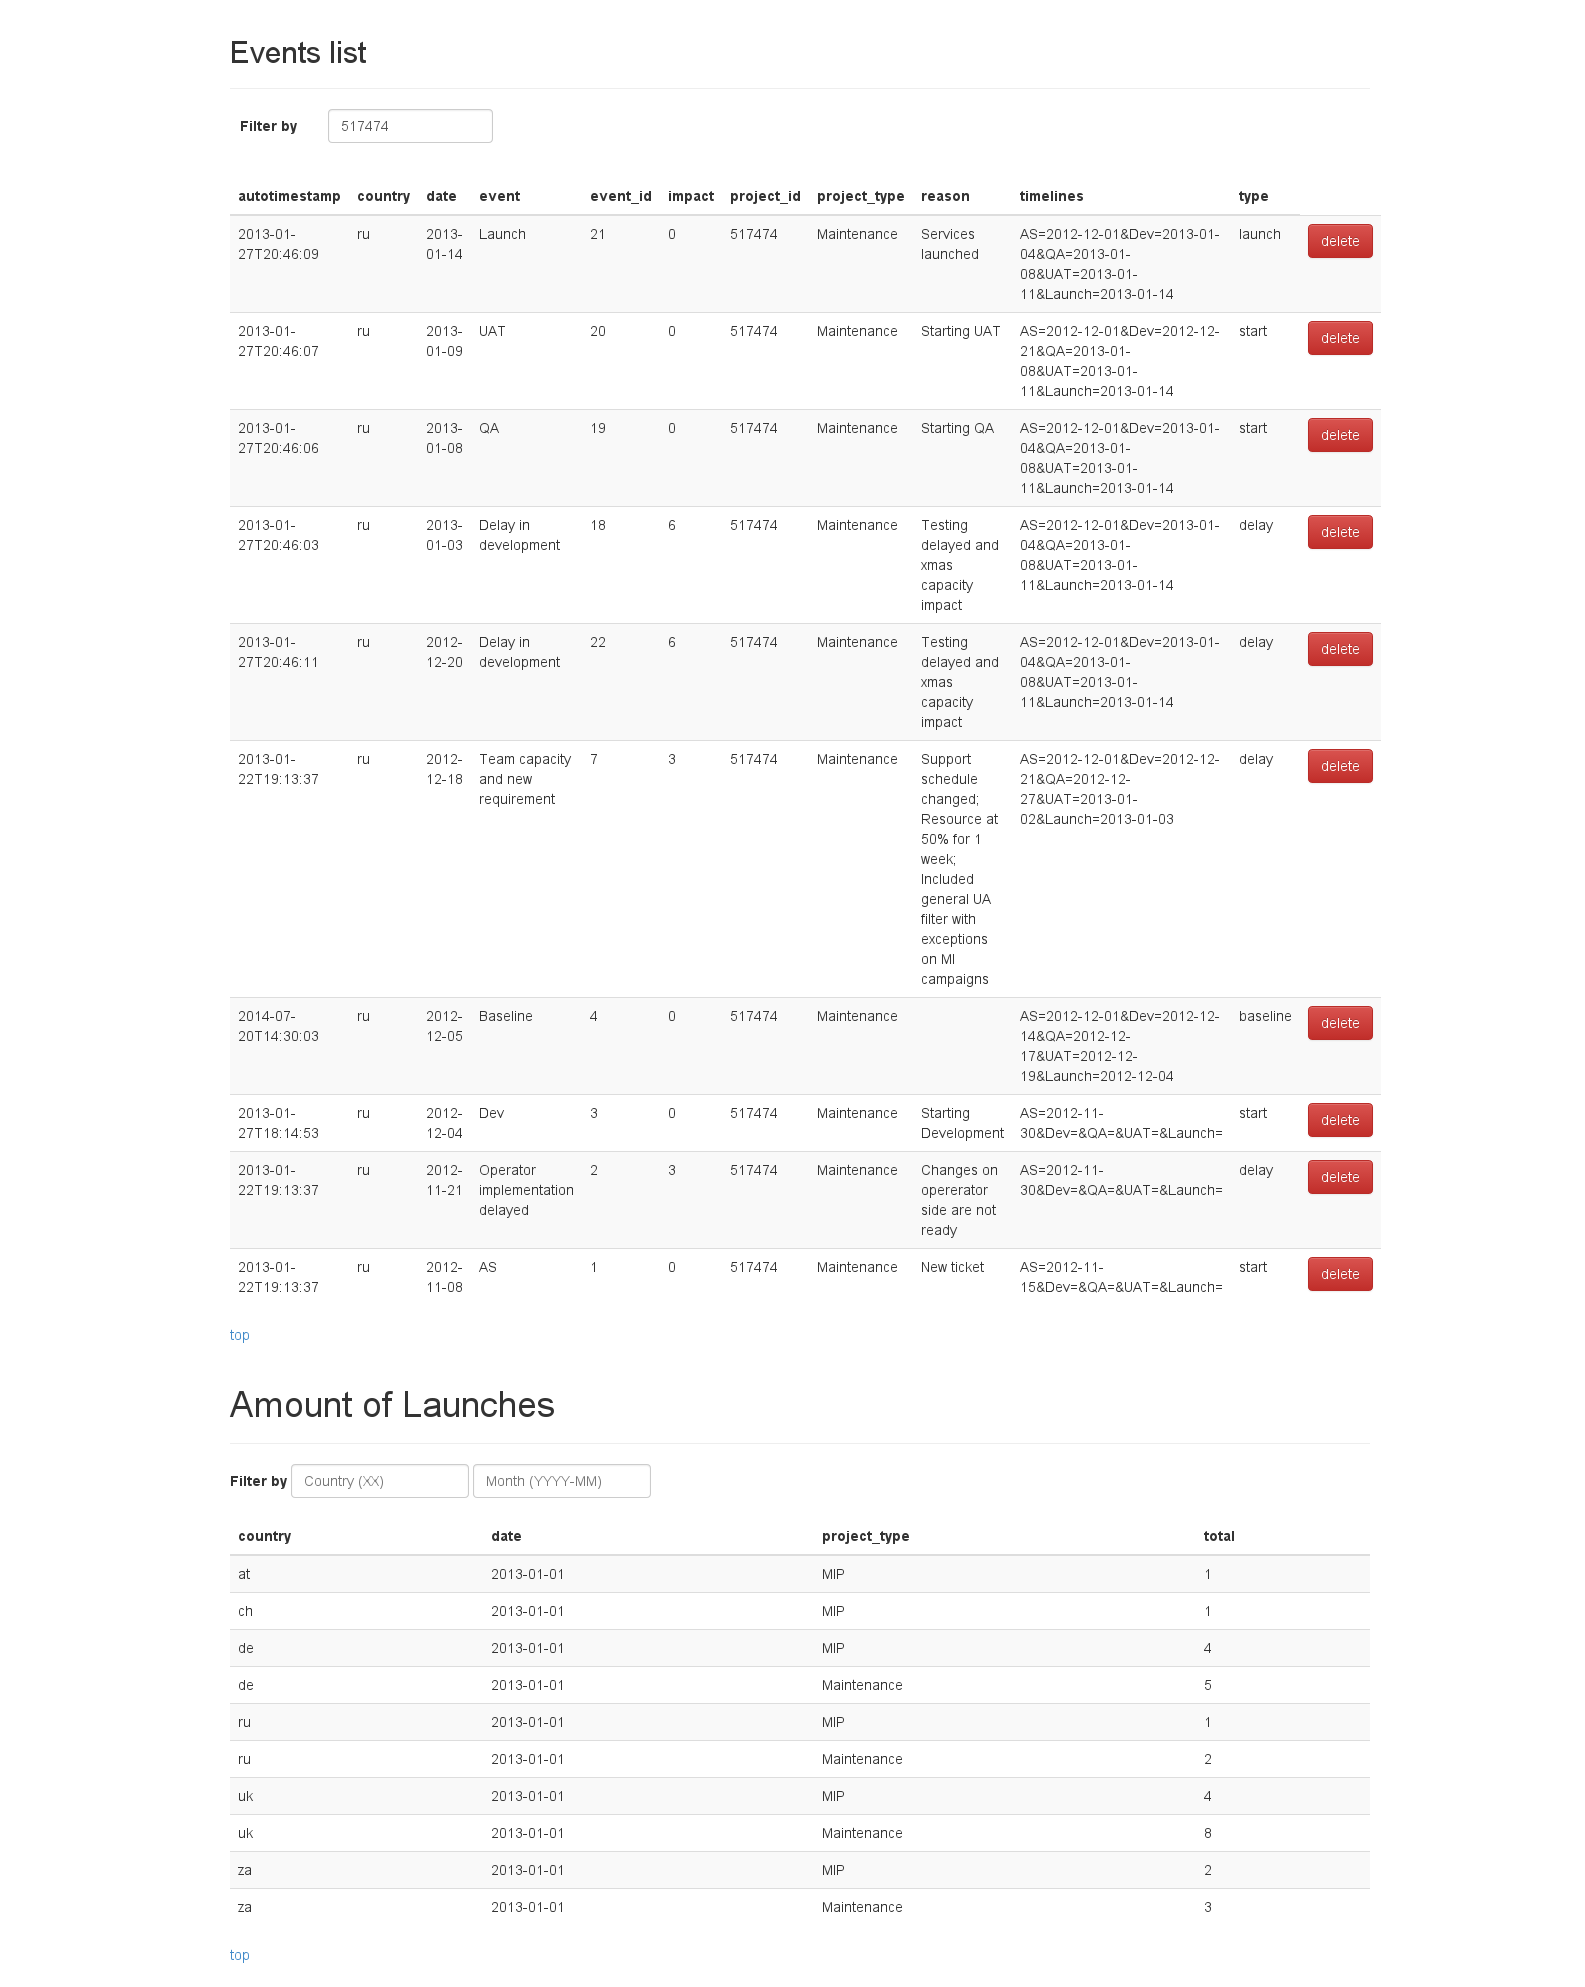
\includegraphics[width=1\textwidth]{./resources/dashboard_after_bootstrap_2.png}
   	\caption{Dasboard look and feel after apply Bootstrap style sheet (2)}
   	\label{f_facelift_bootstrap_2}
\end{figure}

\begin{figure}[ht!]
	\centering
   	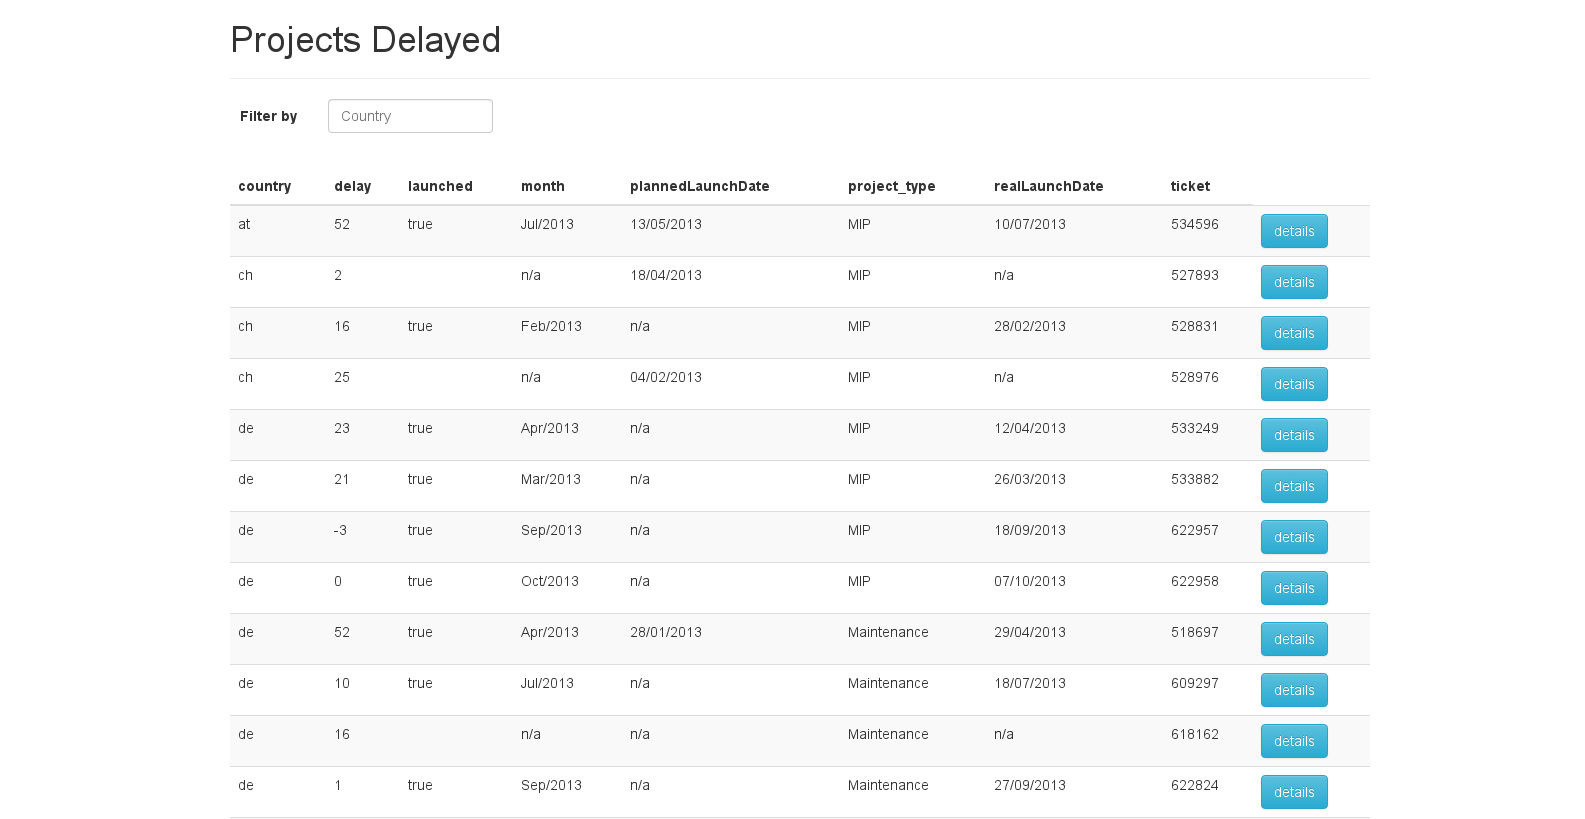
\includegraphics[width=1\textwidth]{./resources/dashboard_after_bootstrap_3.png}
   	\caption{Dasboard look and feel after apply Bootstrap style sheet (3)}
   	\label{f_facelift_bootstrap_3}
\end{figure}

\chapter{Interactive Timelines}
Now we have a responsive and coherent look and feel, we want to be able to
update timelines using directly the timeline chart instead of using 
(\ref{sec:eventlist}) form, that could be less user friendly.

At this stage the first thing we do is to review the API looking for a
\emph{interactive} feature that allows us to implement the respective events to
extend or move an event, as well as change their inherent properties like event
type or description.

The main issue we faced was that Google chart doesn't allow any interaction on
the elements shown, as they are the result of the data already processed, so if we
want to update it we need to update the data and refresh it. But, instead allows
us to customize the \emph{tooltip} object, being able to add an \emph{action},
where we could implement the logic we want
somehow\footnote{\url{https://developers.google.com/chart/interactive/docs/customizing_tooltip_content?hl=es#tooltip_actions}}.

After trying it few times on our Timeline chart and read carefully the
documentation, turns out this Tooltip feature is not available for our specific
type of chart. Also there is open an issue requesting the same logic on
timelines chart
(\url{https://code.google.com/p/google-visualization-api-issues/issues/detail?id=1320}),
so is not feasible to keep using Google charts if we want to have an interactive
timeline chart. Because of that, we started to look for alternatives, and one of
the alternatives found is \emph{CHAP Links
Library}\footnote{\url{http://almende.github.io/chap-links-library/}}, that
provides an interactive timelines chart and has been developed as Google
Visualization Chart, so compatible with what we have implemented till now.

\section{Applying CHAP Timeline chart}
In order to update our tool with the new library and timeline chart, we just
need to download the library and related resources (timeline-2.9.0.zip) and
adjust our html code having reference to it:

\begin{lstlisting}[style=html,breaklines=true,caption=CHAP\ Link\
library,label=f_interactivetimelines_code]
<!-- CHAP Timeline charthttp://almende.github.io/chap-links-library/timeline.html -->
<script type="text/javascript" src="timeline/timeline.js"></script> 
<link rel="stylesheet" type="text/css" href="timeline/timeline.css">
<!-- CHAP Timeline chart -->
\end{lstlisting} 

Once we have the proper JS library loaded and the related CSS together with the
rest of the resources included on the zip file, we proceed to adapt our data to
the new chart.

As mentioned before, this library is compatible with Google Visualization
Chart, that means that we can use \texttt{google.visualization.DataTable}
objects to define the data, in the same way  than before, the only small change
we need to do is to rename column names based  on the on the new library API as
shown on the 
\reffigure{f_interactivetimelines_code}

\begin{lstlisting}[language=Javascript,breaklines=true,caption=CHAP\ Link\
library,label=f_interactivetimelines_code]
var container = document.getElementById('timelinePlot');
var chart = new google.visualization.Timeline(container);
var dataTable = new google.visualization.DataTable();

dataTable.addColumn({ type: 'date', id: 'start' });
dataTable.addColumn({ type: 'date', id: 'end' });
dataTable.addColumn({ type: 'string', id: 'content' });
dataTable.addColumn({ type: 'string', id: 'group' });
dataTable.addColumn({ type: 'boolean', id: 'editable' });
dataTable.addColumn({ type: 'string', id: 'className' });
\end{lstlisting} 

Where:
\begin{itemize}
  \item \texttt{group}: indicates the project that enclosed the event, this is
  because we have more than one event per project.
  \item \texttt{editable}: a flag that enables or disables the editable feature
  for a specific event within the chart using the mouse.
  \item \texttt{className}: field that allows us to set a specific style to this
  element.
\end{itemize}

On the following \reffigure{f_timeline_chap} you can see the style is mostly the
same to the one built using Google charts \reffigure{f_timeline_google},
but the graph generated with CHAP Links allows us to interact with:
\begin{itemize}
  \item Time scale: we can zoom in or out
  \item Add new event
  \item Delete present events
  \item Update starting and ending date for each event
\end{itemize}

\begin{figure}[ht!]
	\centering
   	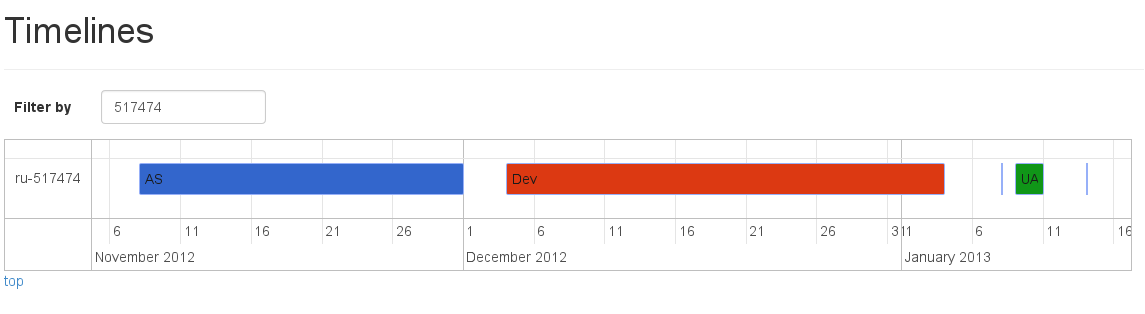
\includegraphics[width=1\textwidth]{./resources/timeline_chap.png}
   	\caption{Timelines chart using CHAP Links API}
   	\label{f_timeline_chap}
\end{figure}

\begin{figure}[ht!]
	\centering
   	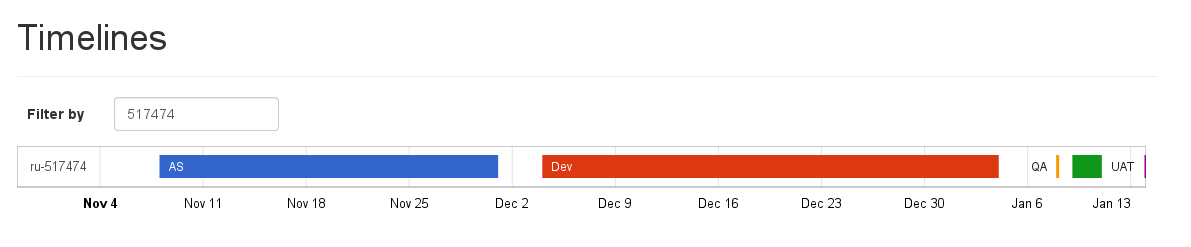
\includegraphics[width=1\textwidth]{./resources/timeline_google.png}
   	\caption{Timelines chart using Google Visualization Chart API}
   	\label{f_timeline_google}
\end{figure} 

This interaction can be processed implementing the right listeners, in our case
we just implement a simple listener that creates a new Event informing the new
dates. The way to do it is just bulding on code the form fields required and
call the same method used on \reffigure{f_migration_addnewevent_jquery}, but
refactored in order to be used by the form and by the chart.

\begin{lstlisting}[language=Javascript,breaklines=true,caption=CHAP On\
change\ event,label=f_interactivetimelines_onchange_code] 
timeline = new links.Timeline(container);
	
// callback function for the change event
var onchanged = function (event) {
    // retrieve the changed row
    var row = getSelectedRow();
    console.debug(timeline.getSelection());
    if (row != undefined) {
        var today = new Date();
        var currentData = data[row];
        var row = timeline.getItem(row);
        var data2create = new Array();
        
        data2create.push({'name':'project_id', 'value': currentData['ticket']});
        data2create.push({'name':'country', 'value': currentData['country']});
        data2create.push({'name':'event', 'value': currentData['phase']});
        data2create.push({'name':'type', 'value': 'info'});
        data2create.push({'name':'project_type', 'value': 'Maintenance'});
        data2create.push({'name':'impact', 'value': 0});
        data2create.push({'name':'reason', 'value': ''});
        data2create.push({'name':'date', 'value': today.getFullYear() +"-"+ today.getMonth()+1 +"-"+ today.getDate()});
        data2create.push({'name':'timelines', 'value': row['end']});
        
        createEvent(currentData["ticket"], data2create);
    }
};

google.visualization.events.addListener(timeline, 'changed', onchanged);
\end{lstlisting} 

Note that the code implemented and shown on \ref{f_interactivetimelines_onchange_code} is not 100\% correct, as
it is using static values, while they should be dynamic ones (like \texttt{project\_type} or
\texttt{type}), and \texttt{timelines} value should be process and well informed
based on original event. But it will be solved on the future work, as it will
require a deep refactoring on the data model, as the graph is the result of
calculating small events in order to build the proper phases and the client is
only aware about the final result (start date and end date).


% \chapter{Extending Dashboard with Elasticsearch and Kibana}
% Working on this currently and see if is feasible to implement the searching and
% data calculation required for the reports based on Elasticsearch. The
% main interesting point here is that we can change the way that we have been
% thinking about the data on this project, and switch it from a relational data
% model (MySQL), to a noSQL approach using Document model (JSON), something that our
% application already uses :)
% 
% Don't know where it will end, but let's see and have fun with it along the
% process.

